\chapter[Estudo de Caso]{Estudo de Caso}

O estudo de caso é uma pesquisa sobre um contexto que seja representativo de um todo. \cite{cervo}

\section[Software BrainBot]{Software BrainBot}

Esta seção apresenta o design e desenvolvimento do Software BrainBot cujo objetivo principal é o de fornecer informação relevante
a respeito de mudanças de tendência no Mercado de Moedas para o par de negociação ouro-dólar.

\subsection[Restrições do Estudo]{Restrições do Estudo}

O coração do software BrainBot consiste numa rede neural recorrente, cuja característica peculiar é que seus nós de processamento possuem
um mecanismo de feedback fazendo com que suas saídas sejam além de entradas para a próxima camada, entradas para o próprio nó fazendo o que
é chamado de loop temporal.

A figura 12 mostra um quadro esquemático de como ficou a rede neural:

\begin{figure}[h]
	\centering
	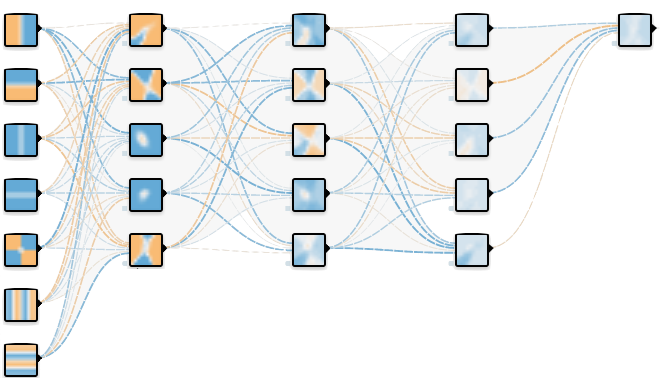
\includegraphics[keepaspectratio=true,scale=0.5]{figuras/desenho.png}
	\caption{Rede Neural - BrainBot - Simulação \cite{tensor}}
	\label{fig12}
\end{figure}

O software BrainBot foi desenhado contendo:

\begin{itemize}
  \item 1 camada de entrada composta de 7 nós
  \item 3 camadas de processamento, cada uma apresentando 5 nós
  \item 1 camada de saída contendo 1 único nó
\end{itemize}

Como foi retratado na figura 12.

A escolha da quantidade de camadas e de nós foi feita levando em consideração \cite{tay}, que cita alguns métodos diferentes:

\begin{itemize}
  \item Tentativa e Erro: Método mais primitivo de escolha, entretanto deve-se ter cuidado pois não é incomum a escolha de estruturas sub-ótimas, principalmente quando a seleção é feita por pessoal inexperiente
	\item Pesquisa Heurística: O objetivo desta análise é elaborar uma fórmula capaz de estimar o número de nós das camadas em função
	do número de entradas e saídas. Esta estimativa pode assumir a forma de uma única topologia ou de uma gama de topologias que devem ser pesquisadas.
	Na prática este método é geralmente utilizado em conjunto com o método de tentativa e erro, funcionando como ponto de partida para a busca subsequente por tentativa e erro.
	\item Busca Exaustiva: Uma busca exaustiva é bastante complicada pelo fato das redes neurais produzirem resultados diferentes de acordo com suas condições
	de inicialização, mesmo quando tudo é mantido fixo.
	\item Algoritmos de Poda e Construção: O objetivo deste método é elaborar uma estrutura eficiente, adicionando e removendo pesos em uma rede neural. \cite{hassibi} faz uma comparação de algoritmos comuns e as diferentes eficiências encontradas.
	Um algoritmo de poda bastante utilizado é o de Dano Cerebral Ideal \cite{yann} que tenta remover progressivamente o peso que causa o menor aumento no erro de treinamento da rede neural.
\end{itemize}

Com o objetivo de restringir e simplificar a abrangência do presente estudo, foi utilizada a estratégia de Tentativa e Erro, utilizando o software TensorFlow que é uma blibioteca de código aberto
para aprendizado de máquina. Consiste num ambiente para treinamento e criação de redes neurais e é desenvolvido e utilizado pelo Google, tanto na área de pesquisa quanto na área de produção. É a segunda
geração do software projetado pelo Google Brain. \cite{tensor}

\pagebreak

\subsubsection[Camada de Entrada]{Camada de Entrada}

O software possui uma camada de entrada, em que cada nó corresponde a uma váriavel distinta dentro do contexto escolhido, daí
a composição dos 7 nós de entrada.

Para alimentar as camadas de entrada foram escolhidas algumas entradas importantes no mercado de moedas, são elas:

\begin{itemize}
  \item Valor de entrada do Mercado
  \item Valor mais alto
  \item Valor de fechamento do Mercado
  \item Valor mais baixo
  \item Média móvel com período 9
  \item Estocástico
  \item Amplitude de Variação
\end{itemize}

Esses valores servem de insumo para a rede neural e são processados nas 3 camadas de processamento e na camada de saída.

Para a escolha das variáveis utilizadas na rede, foram levadas em consideração, as variáveis abordadas em \cite{tau}.
Estudo que aborda influências no Mercado e a Examinação de Variáveis Econômicas. 

O código da camada de entrada pode ser visualizado no link  \href{https://github.com/matmello/brainbot/tree/master/input}{Camada de Entrada}


\subsubsection[Camada de Saída]{Camada de Saída}

A camada de saída é composta por um único nó que corresponde a saída processada pelo software, que é a previsão para o próximo valor
de fechamento na janela de tempo escolhida, no caso deste estudo de caso é a previsão da cotação do Ouro, comprado com dólar para a
próxima hora.

Na camada de saída é utilizada a função retificadora (evidenciada na imagem a seguir) para fornecer valores contínuos representando a respectiva cotação prevista.
\pagebreak
\begin{figure}[h]
	\centering
	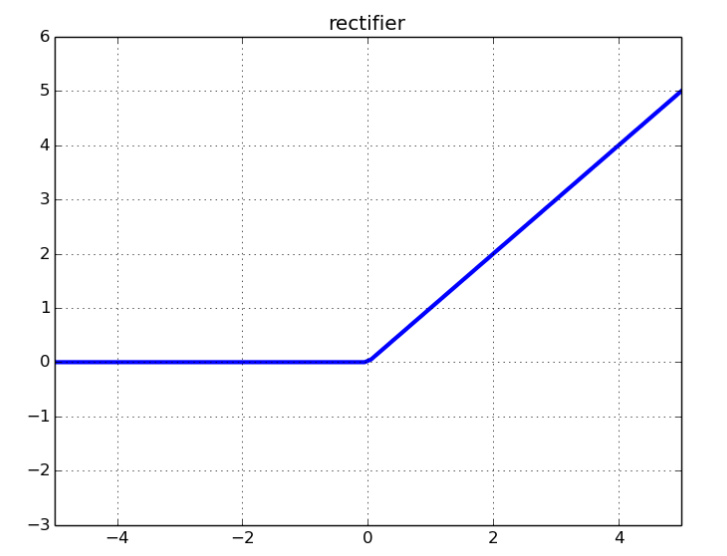
\includegraphics[keepaspectratio=true,scale=0.5]{figuras/ret.png}
	\caption{Função Retificadora \cite{data}}
	\label{fig14}
\end{figure}

O código da camada de saída pode ser visualizado no link  \href{https://github.com/matmello/brainbot/tree/master/output}{Camada de Saída}


\subsubsection[Camada de Processamento]{Camada de Processamento}


São utilizadas dois tipos de funções de ativação no funcionamento dos nós de processamento.

A primeira função utilizada em alguns nós de processamento é a função treshold que pode ser vista na figura seguinte:

\pagebreak

\begin{figure}[h]
	\centering
	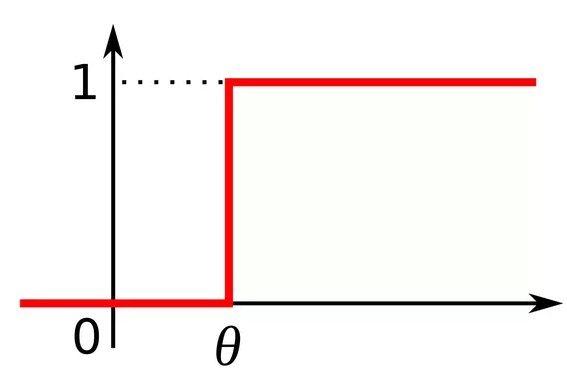
\includegraphics[keepaspectratio=true,scale=0.6]{figuras/tresh.png}
	\caption{Função Treshold \cite{data}}
	\label{fig13}
\end{figure}

A função acima é utilizada para fornecer valores binários como saída dos nós de processamento em que é utilizada.

A segunda função que é utilizada nos nós de processamento restantes é a função retificadora, da mesma maneira em que é utilizada nos
nós de saída do software.

O código da camada de processamento pode ser visualizado no link  \href{https://github.com/matmello/brainbot/tree/master/hidden}{Camada de Processamento}


\subsection[Desenvolvimento]{Desenvolvimento}

Para o desenvolvimento do sistema foi utilizado o seguinte ambiente:

\begin{itemize}
  \item Python versão 3.6.2
  \item IDE Spyder versão 3.1.4
  \item Sistema operacional OSX versão Sierra
  \item Editor de texto Atom
\end{itemize}

Após o desenho do sistema e do funcionamento de cada nó, com suas entradas e seu processamento. Os nós foram desenvolvidos
um a um, começando pelos nós de entradas cuja principal função é padronizar as entradas, até o nó de saída que fornece o valor previsto
de fechamento para a próxima cotação do par de negociação utilizado.

Cada nó de processamento foi considerado como uma história de usuário e cada rotina de processamento como por exemplo o tratamento dos dados
foi considerado como tarefa.

\section[Desenho do Estudo de Caso]{Desenho do Estudo de Caso}

\subsection[Coleta de Dados]{Coleta de Dados}

Para a coleta de dados foram utilizadas as variáveis definidas anteriormente, considerando o par de negociação ouro-dólar, os valores entre
as datas: 01/01/2013 e 27/09/2015 foram utilizados para treinar a rede neural. A janela de tempo utilizada foi de uma hora e o número de ciclos de aprendizado foi de 50, 100, 200 e 300 respectivamente.
Para a contabilização dos resultados, tentou-se prever as cotações entre os dias 27/09/2015 e 10/10/2015.

\subsection[Análise de Dados]{Análise de Dados}

Respeitando o contexto e o ambiente já definido, a rede neural foi executada e os valores coletados. A análise foi feita de forma percentual,
classificando como acerto se a rede neural foi capaz de prever a queda ou subida para a próxima cotação.

\subsection[Validação de Dados]{Validação de Dados}

A validade do estudo foi respeitada na forma da integridade dos dados que apresentam além das variáveis determinadas, dados do tempo em que
as medições foram aferidas.
Para aumentar a confiabilidade do estudo foram feitas três medições para cada ciclo de aprendizado definido e os dados resultados foram registrados.

\section[Análise e Interpretação dos Resultados]{Análise e Interpretação dos Resultados}

Os resultados foram divididos conforme a quantidade de ciclos de aprendizado aplicados.

\pagebreak

\subsection[50 Ciclos]{50 Ciclos}

Utilizando 50 ciclos de aprendizado obteve-se os seguintes resultados:

\begin{figure}[h]
	\centering
	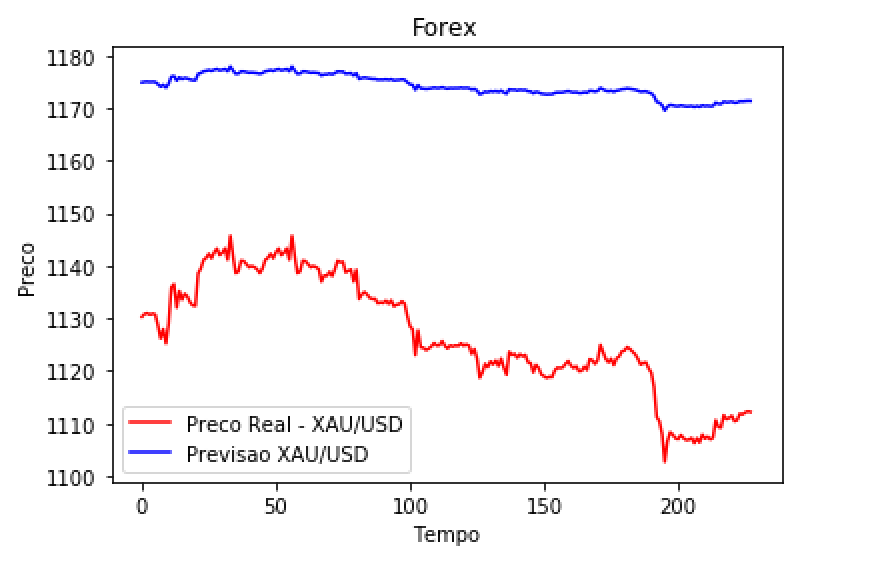
\includegraphics[keepaspectratio=true,scale=0.8]{figuras/50high.png}
	\caption{50 Ciclos}
	\label{fig15}
\end{figure}

A linha azul representa a saída do software e a linha vermelha representa os valores corretos de cotação.

A figura abaixo apresenta uma visão mais detalhada de apenas 8 cotações individuais:

\begin{figure}[h]
	\centering
	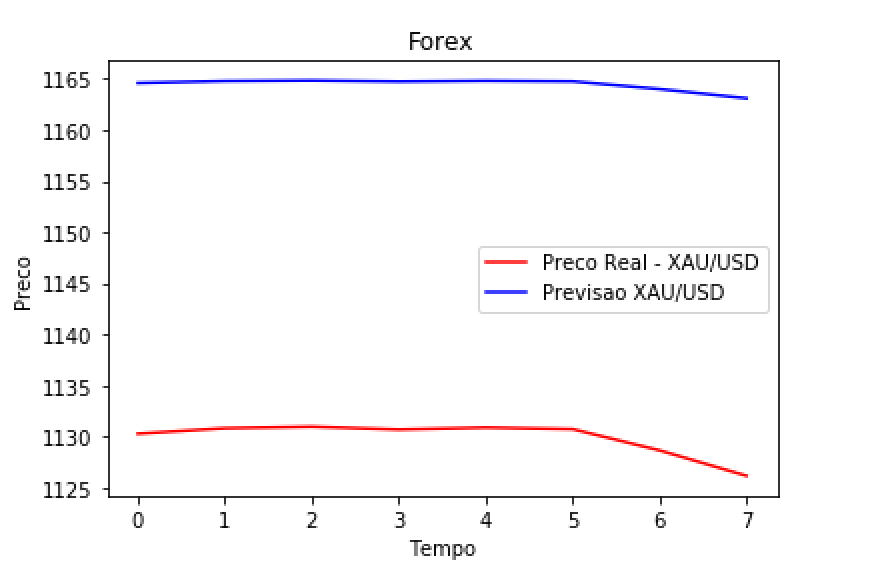
\includegraphics[keepaspectratio=true,scale=0.8]{figuras/50low.png}
	\caption{50 Ciclos}
	\label{fig16}
\end{figure}

Pode-se observar apenas pela observação do gráfico que os resultados obtidos não foram satisfatórios para a previsão de cotações neste
contexto específico, e quaiquer resultados percentuais satisfatórios seriam por pura ocasião. Para o caso de 50 ciclos, foi dispensada
a análise percentual.

\subsection[100 Ciclos]{100 Ciclos}

Os resultados apresentados utilizando 100 ciclos de aprendizado foram relatados a seguir:

\begin{figure}[h]
	\centering
	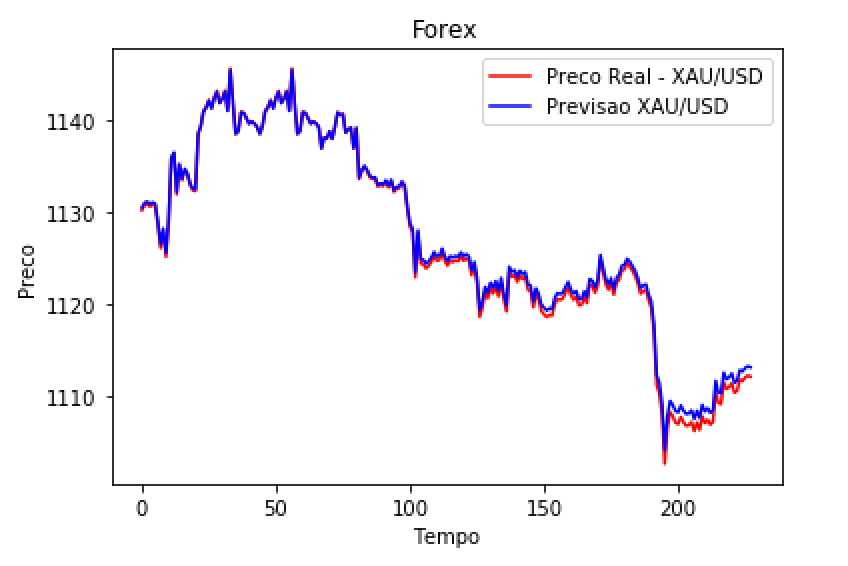
\includegraphics[keepaspectratio=true,scale=0.8]{figuras/100high.png}
	\caption{100 Ciclos}
	\label{fig17}
\end{figure}

Analisando o gráfico acima, percebe-se que os resultados em alto nível se assemelharam ao resultado real, mas a análise percentual
trouxe melhores informações sobre o quão efetivo seria esse contexto em ajudar um negociador no Mercado de Moedas.

\pagebreak

Os dados para apenas 8 observações individuais ( apenas para melhor observação ):

\begin{figure}[h]
	\centering
	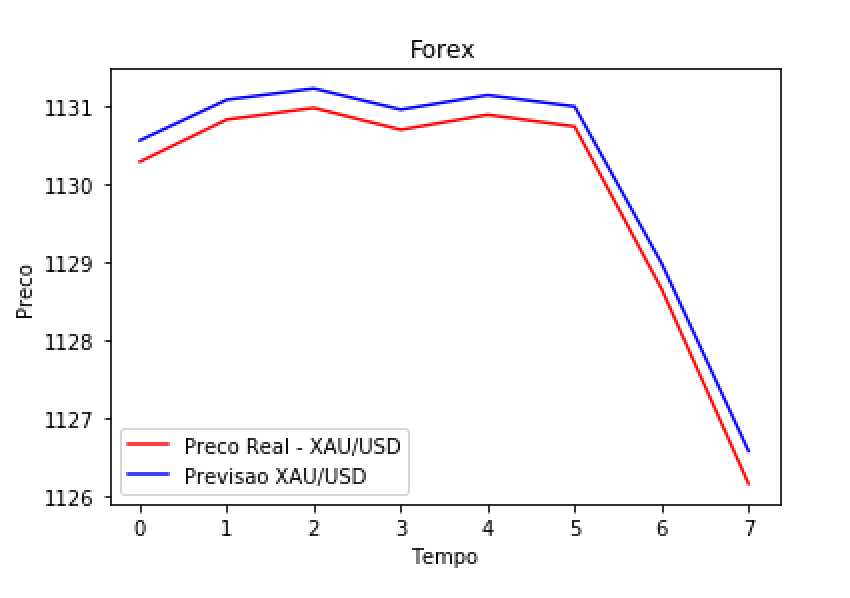
\includegraphics[keepaspectratio=true,scale=0.8]{figuras/100low.png}
	\caption{100 Ciclos}
	\label{fig18}
\end{figure}

A tabela a seguir mostra a análise percentual dos resultados obtidos:

\begin{table}[h]
	\centering
	\caption{Percentual para 100 ciclos}
	\label{tab09}
  \begin{center}
      \begin{tabular}{ | l | p{5cm}}
      \hline
      Ciclos de aprendizado & Percentual de Acerto \\ \hline
		  100 & 48.74 \\ \hline
      \end{tabular}
  \end{center}
\end{table}

Analisando o percentual de acerto quanto a tendência, percebe-se que este contexto também não apresentou resultados satisfatórios, na
medida que se um investigador usasse sua própria intuição talvez obtivesse melhores resultados.

\pagebreak


\subsection[200 Ciclos]{200 Ciclos}

Os resultados apresentados utilizando 200 ciclos de aprendizado foram relatados a seguir:

\begin{figure}[h]
	\centering
	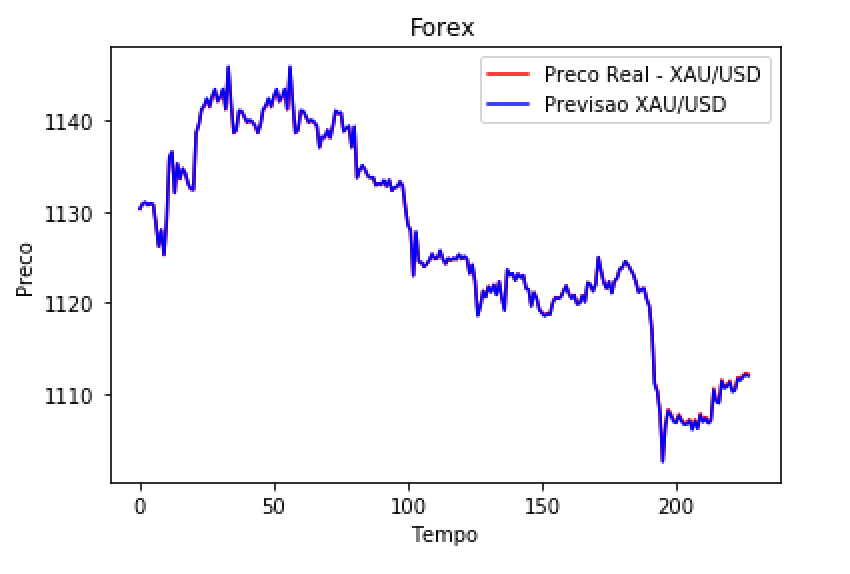
\includegraphics[keepaspectratio=true,scale=0.8]{figuras/200high.png}
	\caption{200 Ciclos}
	\label{fig18}
\end{figure}

Os dados para apenas 8 observações individuais:

\begin{figure}[h]
	\centering
	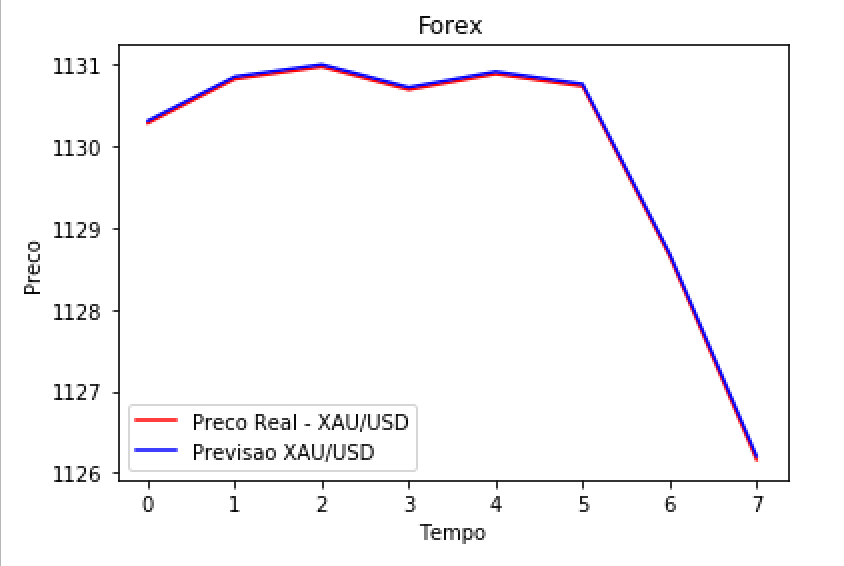
\includegraphics[keepaspectratio=true,scale=0.8]{figuras/200low.png}
	\caption{200 Ciclos}
	\label{fig18}
\end{figure}

\pagebreak

A tabela a seguir mostra a análise percentual dos resultados obtidos:

\begin{table}[h]
	\centering
	\caption{Percentual para 200 ciclos}
	\label{tab10}
  \begin{center}
      \begin{tabular}{ | l | p{5cm}}
      \hline
      Ciclos de aprendizado & Percentual de Acerto \\ \hline
		  200 & 72.8 \\ \hline
      \end{tabular}
  \end{center}
\end{table}

Os resultados utilizando 200 ciclos de aprendizados foram satisfatórios para o contexto definido, a rede neural foi capaz de prever
com 72.8\% de acerto, a tendência correta da próxima cotação.

\subsection[300 Ciclos]{300 Ciclos}

Os resultados apresentados utilizando 300 ciclos de aprendizado foram relatados a seguir:

\begin{figure}[h]
	\centering
	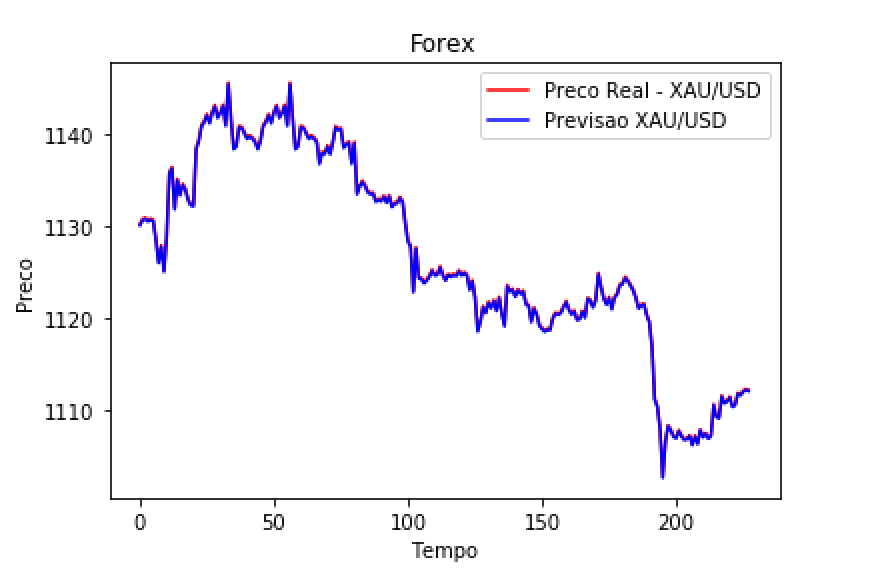
\includegraphics[keepaspectratio=true,scale=0.8]{figuras/300high.png}
	\caption{300 Ciclos}
	\label{fig18}
\end{figure}

Os dados para apenas 8 observações individuais:

\begin{figure}[h]
	\centering
	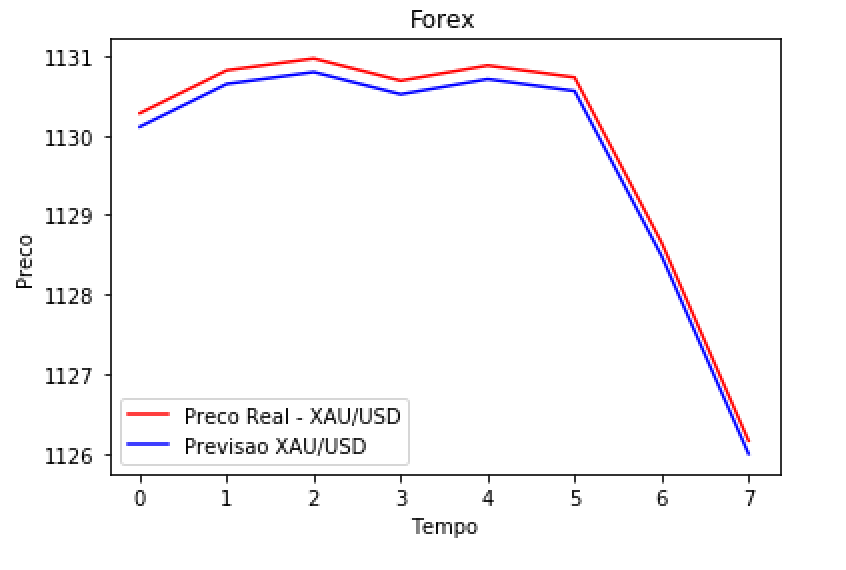
\includegraphics[keepaspectratio=true,scale=0.8]{figuras/300low.png}
	\caption{300 Ciclos}
	\label{fig18}
\end{figure}

\pagebreak

A tabela a seguir mostra a análise percentual dos resultados obtidos:

\begin{table}[h]
	\centering
	\caption{Percentual para 300 ciclos}
	\label{tab10}
  \begin{center}
      \begin{tabular}{ | l | p{5cm}}
      \hline
      Ciclos de aprendizado & Percentual de Acerto \\ \hline
		  300 & 60.1 \\ \hline
      \end{tabular}
  \end{center}
\end{table}

Os resultados neste contexto foram razoavelmente satisfatórios, mas apresentaram efetividade menor do que se comparado com a amostra de 200 ciclos.

\pagebreak
